\documentclass[11pt]{article}

\usepackage[utf8]{inputenc}
\usepackage[T1]{fontenc}
\usepackage[english]{babel}
\usepackage{amsmath,amssymb}
\usepackage{graphicx}
\graphicspath{{figures/}}
\usepackage{booktabs}
\usepackage{geometry}
\geometry{a4paper,margin=2.6cm}
\usepackage[round]{natbib}
\usepackage[hidelinks]{hyperref}
\usepackage{abstract}

\title{\textbf{On the inevitability of a homicidal ancestor:\\
a genealogical--probabilistic argument}}
\author{Juan Manuel Lemos\\
\normalsize Independent researcher\thanks{Author's note: this work arises from a
personal inquiry driven by curiosity; it is offered as a rigorous and
reproducible synthesis, in a scientific spirit, without claiming academic
credentials.}}
\date{\today}

\begin{document}
\maketitle

\begin{abstract}
\noindent We start from an existential question: \emph{what is the probability
that neither I nor any of my ancestors ever caused the death of another human
being?} We formalise this as a problem of compound probability over the
ascending genealogical tree. We show that, because of the exponential growth in
the number of ancestors, this probability collapses to values indistinguishable
from zero within a few dozen generations, even under extremely conservative
assumptions about the prevalence of lethal violence. Moreover, invoking the
\emph{identical ancestors point} \citep{rohde2004}, the argument ceases to be
probabilistic and becomes essentially deductive: beyond that horizon, the set of
ancestors of any living person coincides with the entire global breeding
population of that era, so that the existence of a single killer in that pool
suffices. We support the result with a Monte Carlo simulation, and we examine
isolated populations and the relaxation of the independence assumption. We
conclude that it is practically impossible not to descend from at least one
killer.
\end{abstract}

\section{Introduction}

Many people intuit that their lineage could have been free of lethal violence:
``not I, not my parents, not my grandparents, nobody back through time''. This
note shows that such an intuition is mathematically untenable. The argument does
not rest on assuming that humans are especially violent, but on a purely
combinatorial property of kinship: the number of ancestors grows exponentially
into the past, and a logical conjunction (``\emph{no one} was a killer'') over an
enormous number of individuals becomes, in practice, impossible to satisfy.

We combine three ingredients: (i) a naive model of the doubling of ancestors;
(ii) the correction due to \emph{pedigree collapse}; and (iii) the
\emph{identical ancestors point} (IAP), which turns the probabilistic result
into a practical certainty.

\section{Definitions and assumptions}\label{sec:def}

\paragraph{Killer.} We adopt a broad and deliberate definition: a person is a
\emph{killer} if they caused the death of another human being by any intentional
or quasi-intentional cause (war, self-defence, intergroup conflict, etc.). This
choice maximises the robustness of the argument and avoids the legal and moral
ambiguities that depend on the era.

\paragraph{Ancestor.} We use the \emph{genealogical} (lineal) sense: every
parent, grandparent, great-grandparent, etc., regardless of whether or not they
transmitted genetic material to the descendant. The distinction between
genealogical and genetic ancestry is relevant and is discussed in
Section~\ref{sec:disc} \citep{ralph2013}.

\paragraph{Parameters.} Let $p$ be the probability that any given individual is a
killer over their lifetime, and $q = 1-p$. Let $N$ be the number of generations
considered into the past and $\ell \approx 28$ years the mean generation length
\citep{fenner2005}.

\paragraph{Independence assumption.} In the analytic models we assume that the
events ``being a killer'' are independent across individuals. This is a
simplification (there is family and regional correlation); its effect is examined
in Section~\ref{sec:disc} and relaxed in the simulation.

\section{Probabilistic model}

\subsection{Naive model}

The number of ancestors doubles each generation: $2$ parents, $4$ grandparents,
\dots, $2^n$ at generation $n$. The total number of individuals in the lineage
(including \emph{ego}) up to generation $N$ is
\begin{equation}
  T(N) \;=\; \sum_{k=0}^{N} 2^k \;=\; 2^{\,N+1}-1 .
\end{equation}
Under independence, the probability that \emph{none} of them is a killer is
\begin{equation}\label{eq:naive}
  P_{\text{naive}}(p,N) \;=\; (1-p)^{\,T(N)} \;=\;
  \exp\!\big[(2^{\,N+1}-1)\,\ln(1-p)\big].
\end{equation}
Since $T(N)$ grows exponentially, for any fixed $p>0$ we have
$P_{\text{naive}}(p,N)\to 0$ very quickly (Fig.~\ref{fig:naive}).

\subsection{Pedigree collapse}

The naive model overcounts: the ``slots'' $2^n$ soon exceed the human population
of the era, so a single individual occupies many positions of the tree
(\emph{pedigree collapse}). The number of \emph{distinct} ancestors at generation
$n$ is bounded by the breeding population $\Pi(n)$:
\begin{equation}\label{eq:collapse}
  D(n) \;=\; \min\!\big(2^{\,n},\, \Pi(n)\big).
\end{equation}
Saturation occurs around $n^\star = \lceil \log_2 \Pi \rceil$. For
$\Pi \sim 10^{8}$, $n^\star \approx 27$ ($\sim 750$ years); for
$\Pi \sim 8\times 10^{9}$, $n^\star \approx 33$ ($\sim 920$ years)
(Fig.~\ref{fig:collapse}). Far from rescuing the intuition, collapse
\emph{worsens} it: beyond $n^\star$ the ancestors of \emph{ego} are practically
the entire population of their era.

\subsection{Identical ancestors point (the strong argument)}

\citet{chang1999} showed that, in a well-mixed population of size $N_e$, one need
only go back of order $1{.}77\,\log_2 N_e$ generations for every individual of
that time (with descendants today) to be an ancestor of \emph{all} the present
population. \citet{rohde2004} estimated, by simulation with realistic migration,
that the most recent common ancestor (MRCA) of \emph{Homo sapiens} lived
$\sim 2\,000$--$5\,000$ years ago, and that the \emph{identical ancestors point}
(IAP) ---the moment beyond which every person of that time with descendants is an
ancestor of all the living--- lies, depending on the mixing assumptions,
approximately $5\,000$--$15\,000$ years ago (with bounds of $1\,000$--$15\,000$
years in more conservative estimates).

The consequence is decisive. Let $\mathcal{E}$ be the global breeding population
at an era prior to the IAP, of size $|\mathcal{E}|$. Beyond the IAP, \emph{the set
of ancestors of any living person is exactly $\mathcal{E}$}. Therefore, the
probability of descending from at least one killer is
\begin{equation}\label{eq:iap}
  P_{\text{desc}}(p) \;=\; 1-(1-p)^{\,|\mathcal{E}|}.
\end{equation}
With $|\mathcal{E}|$ of order millions (or billions), an infinitesimal $p$
suffices for $P_{\text{desc}}(p)\approx 1$ (Table~\ref{tab:iap}). The statement
ceases to be probabilistic: if at least one killer \emph{existed} in $\mathcal{E}$
---something empirically certain (Section~\ref{sec:param})--- then \emph{every}
living human descends from a killer.

\section{Empirical parameters}\label{sec:param}

To fix $p$ we use as an anchor the phylogenetic analysis of \citet{gomez2016}:
the proportion of human deaths \emph{predicted} by comparative methods to be due
to interpersonal violence is $\approx 2\%$, a value consistent with that inferred
for the evolutionary ancestor of primates and with that observed in prehistoric
bands and tribes (and exceeded in many historical periods). In an approximately
stationary population, each violent death implies at least one perpetrator, so
the fraction of people who ever killed is of the same order of magnitude:
$p \sim 10^{-2}$. Considering war and intergroup conflict over millennia, $p$
could be substantially higher. As a precaution, we explore a wide range
$p \in [10^{-4},\, 0{.}15]$ and show that the conclusion holds even at its lower
end.

As a bound on the number of individuals involved, we use the estimate that
$\sim 1{.}17\times 10^{11}$ human beings have ever been born \citep{prb2022}
(other estimates give $\sim 1{.}08\times 10^{11}$); the number of \emph{distinct}
ancestors of any person is bounded by this figure. For the size of the breeding
population in each era we use the long-run demographic series of
\citet{owid2023population}.

\section{Results}

\paragraph{Naive model.} Table~\ref{tab:naive} and Fig.~\ref{fig:naive} show the
collapse of $P_{\text{naive}}(p,N)$. Already at $N=15$ generations
($\sim 420$ years) the probability is astronomically small except for unrealistically
low $p$.

\begin{table}[h]
\centering
\caption{$P_{\text{naive}}(p,N)$: probability that \emph{no} ancestor (naive
model) is a killer.}
\label{tab:naive}
\begin{tabular}{rrcccc}
\toprule
$N$ & individuals & $p=0{.}001$ & $p=0{.}01$ & $p=0{.}05$ & $p=0{.}15$ \\
\midrule
5  & 63        & $9{.}4\times10^{-1}$ & $5{.}3\times10^{-1}$ & $4{.}0\times10^{-2}$ & $3{.}6\times10^{-5}$ \\
10 & 2\,047    & $1{.}3\times10^{-1}$ & $1{.}2\times10^{-9}$ & $2{.}5\times10^{-46}$ & $3{.}3\times10^{-145}$ \\
15 & 65\,535   & $3{.}3\times10^{-29}$ & $9{.}0\times10^{-287}$ & $\approx 0$ & $\approx 0$ \\
20 & 2\,097\,151 & $\approx 0$ & $\approx 0$ & $\approx 0$ & $\approx 0$ \\
\bottomrule
\end{tabular}
\end{table}

\paragraph{IAP argument.} Table~\ref{tab:iap} evaluates Eq.~\eqref{eq:iap} for a
breeding pool of $|\mathcal{E}| = 5\times 10^{6}$. Even with $p = 10^{-6}$ (one in
a million), the probability of descending from a killer exceeds $0{.}99$; for
$p \ge 10^{-5}$ it is, numerically, equal to $1$.

\begin{table}[h]
\centering
\caption{$P_{\text{desc}}(p) = 1-(1-p)^{|\mathcal{E}|}$ with
$|\mathcal{E}| = 5\times 10^{6}$.}
\label{tab:iap}
\begin{tabular}{cc}
\toprule
$p$ & $P_{\text{desc}}(p)$ \\
\midrule
$10^{-6}$ & $0{.}9933$ \\
$10^{-5}$ & $1{.}0000$ \\
$10^{-4}$ & $1{.}0000$ \\
$10^{-3}$ & $1{.}0000$ \\
$10^{-2}$ & $1{.}0000$ \\
\bottomrule
\end{tabular}
\end{table}

\paragraph{Monte Carlo simulation.} We build a population of $M = 5\,000$
individuals per generation over $30$ generations with random mating; each
individual is a killer independently with probability $p$, and we propagate the
indicator ``has at least one homicidal ancestor'' (average of $20$ replicates).
Even with $p = 10^{-4}$, the fraction of the present population with a homicidal
ancestor reaches practically $1$ by generation~$20$--$29$; with $p = 10^{-2}$, by
generation~$10$ (Table~\ref{tab:sim}). The simulation relaxes the
infinite-population assumption of the naive model and confirms the result.

\begin{table}[h]
\centering
\caption{Fraction of the population with $\ge 1$ homicidal ancestor (Monte
Carlo, $M=5\,000$, $20$ replicates).}
\label{tab:sim}
\begin{tabular}{rccc}
\toprule
generation & $p=10^{-4}$ & $p=10^{-3}$ & $p=10^{-2}$ \\
\midrule
5  & $0{.}006$ & $0{.}060$ & $0{.}460$ \\
10 & $0{.}155$ & $0{.}826$ & $1{.}000$ \\
15 & $0{.}764$ & $1{.}000$ & $1{.}000$ \\
20 & $0{.}998$ & $1{.}000$ & $1{.}000$ \\
29 & $1{.}000$ & $1{.}000$ & $1{.}000$ \\
\bottomrule
\end{tabular}
\end{table}

\begin{figure}[h]
\centering
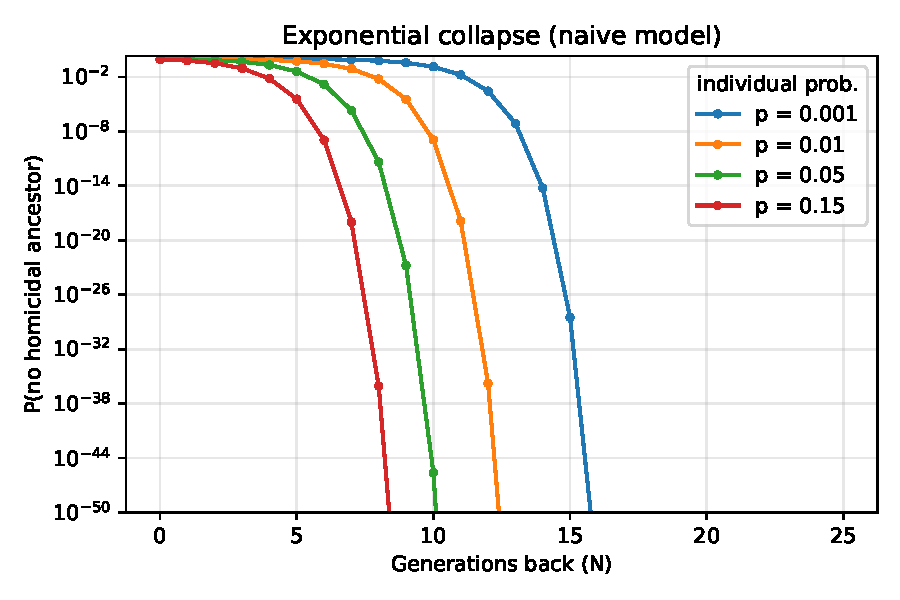
\includegraphics[width=0.72\textwidth]{fig_naive_collapse_en.pdf}
\caption{Exponential collapse of $P_{\text{naive}}(p,N)$ (logarithmic scale)
according to the naive model, Eq.~\eqref{eq:naive}.}
\label{fig:naive}
\end{figure}

\begin{figure}[h]
\centering
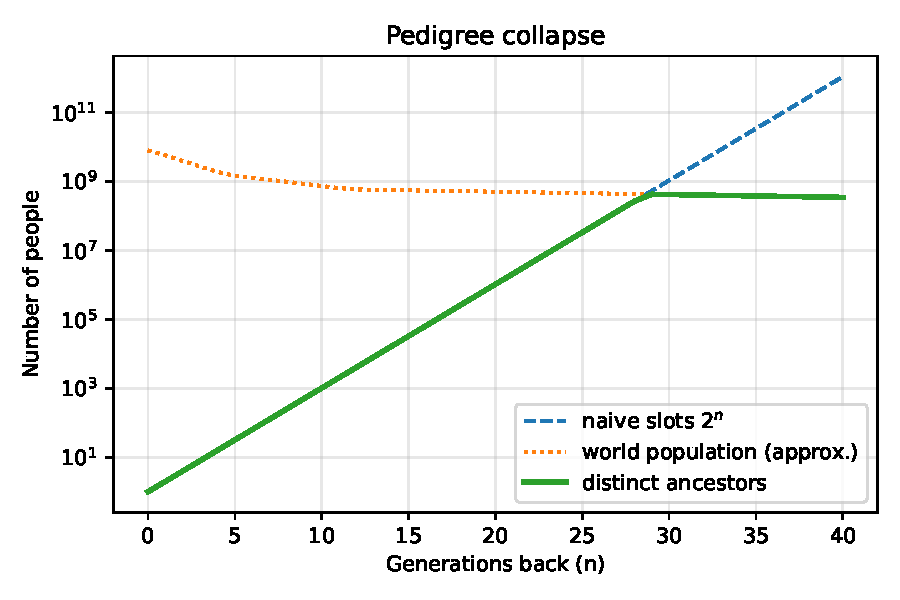
\includegraphics[width=0.72\textwidth]{fig_pedigree_collapse_en.pdf}
\caption{Pedigree collapse: the naive slots $2^n$ exceed the population, so the
distinct ancestors $D(n)$ saturate, Eq.~\eqref{eq:collapse}.}
\label{fig:collapse}
\end{figure}

\begin{figure}[h]
\centering
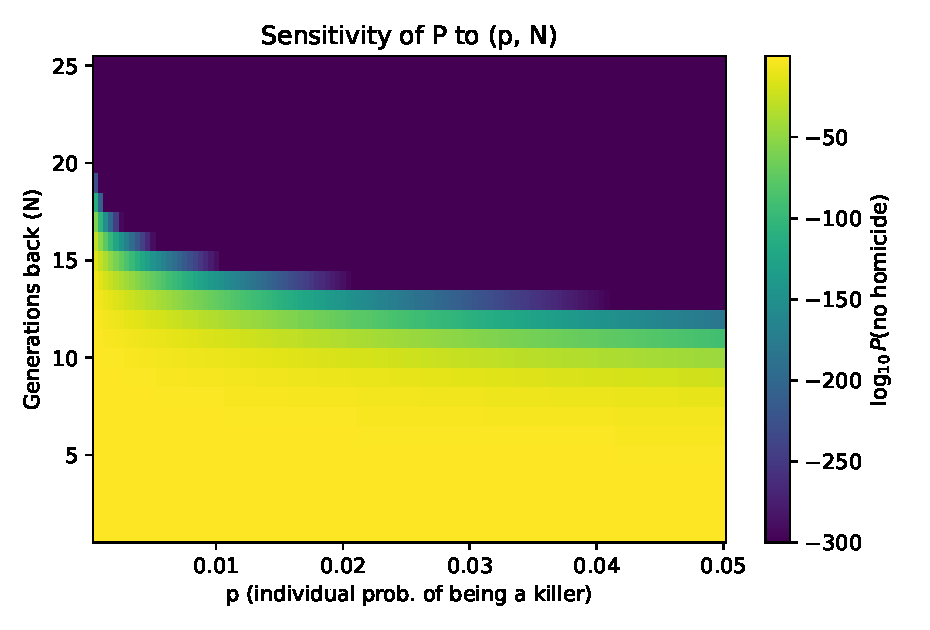
\includegraphics[width=0.72\textwidth]{fig_sensitivity_heatmap_en.pdf}
\caption{Sensitivity of $\log_{10} P_{\text{naive}}$ to $(p,N)$. The dark region
(probability $\approx 0$) dominates except for very small $p$ and very small
$N$.}
\label{fig:heat}
\end{figure}

\section{Discussion and limitations}\label{sec:disc}

\paragraph{Independence.} The independence hypothesis is false: the propensity to
violence correlates within families and regions, and warlike events affect many
at once. However, positive correlation tends to \emph{reinforce} the conclusion
(it concentrates killers in some branches, but a single branch suffices to break
the conjunction), and the random-mating simulation already dispenses with the
infinite population.

\paragraph{Heritability and correlation.} The propensity to violence has a
hereditary and culturally transmitted component \citep{anholt2012}, which
introduces correlation between the status of parents and children. To assess its
effect we extend the simulation with a transmission parameter $h\in[0,1]$,
$p_{\text{child}} = p + h\,(f-p)$, where $f$ is the fraction of the two parents
who were killers; the model \emph{preserves the marginal prevalence} $p$, so it
compares the independent case ($h=0$) with the clustered one ($h>0$) at equal
mean violence. The simulated prevalence stays at $\approx 0{.}010$ for all $h$
(Table~\ref{tab:heritability}), and even with $h=0{.}9$ the fraction with a
homicidal ancestor converges to $1$, crossing $0{.}999$ at generation~$10$ versus
generation~$9$ in the independent case (Fig.~\ref{fig:heritability}). That is,
correlation barely delays the phenomenon by one generation and does not change
the conclusion: the thesis is robust to the independence assumption.

\begin{table}[h]
\centering
\caption{Robustness to independence (Monte Carlo, $p=0{.}01$, $M=2\,000$,
$40$ replicates). $h$ is the heritability/transmission; the marginal prevalence
is preserved.}
\label{tab:heritability}
\begin{tabular}{cccc}
\toprule
$h$ & prevalence & gen.\ with frac.\ $\ge 0{.}999$ & fraction (gen.\ 29) \\
\midrule
$0{.}0$ & $0{.}010$ & $9$  & $1{.}000$ \\
$0{.}3$ & $0{.}010$ & $9$  & $1{.}000$ \\
$0{.}6$ & $0{.}010$ & $10$ & $1{.}000$ \\
$0{.}9$ & $0{.}010$ & $10$ & $1{.}000$ \\
\bottomrule
\end{tabular}
\end{table}

\begin{figure}[h]
\centering
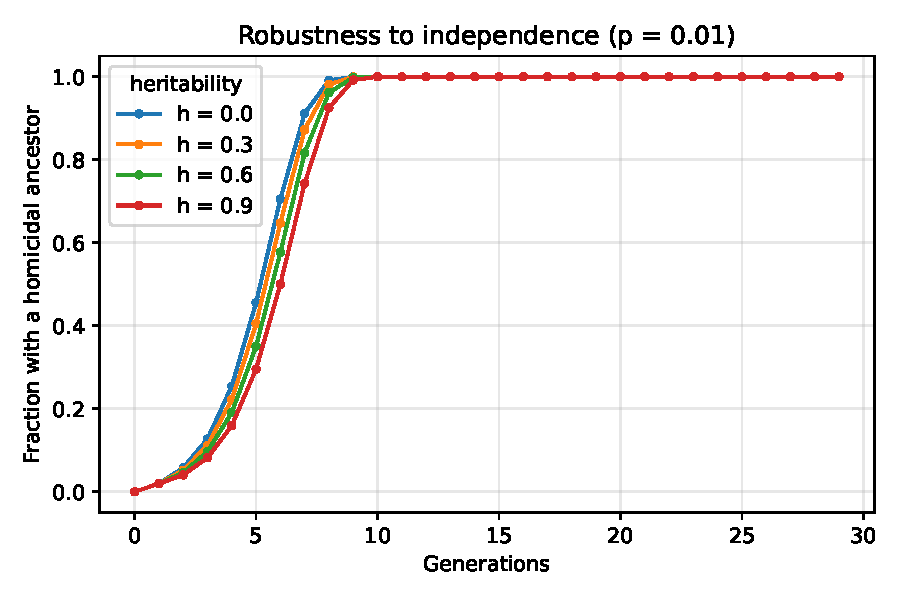
\includegraphics[width=0.72\textwidth]{fig_heritability_en.pdf}
\caption{Robustness to independence: fraction with a homicidal ancestor per
generation for different levels of heritability/correlation $h$, at fixed
marginal prevalence $p=0{.}01$. The curves are almost indistinguishable.}
\label{fig:heritability}
\end{figure}

\paragraph{Genealogical vs.\ genetic.} The argument is \emph{genealogical}. An
ancestor at the IAP may have left no genetic material in \emph{ego}
\citep{ralph2013}. This does not affect the claim about descent, which is
genealogical, not genetic, in nature.

\paragraph{Sensitivity to the definition.} Under a strict legal definition of
``murder'' (unlawful homicide), $p$ would be smaller; even so,
Tables~\ref{tab:iap} and~\ref{tab:sim} show that the result holds for $p$ as low
as $10^{-4}$.

\paragraph{Population mixing.} The model of \citet{rohde2004} assumes global
mixing, mitigated in reality by geographic barriers; this delays the global IAP
but does not eliminate it, and the \emph{regional} IAP is even more recent.

\paragraph{Isolated populations.} One might ask whether an isolated population
(an island, a remote valley, a settlement founded by a few colonists) could
escape the conclusion. The analysis shows the opposite, in three ways. (i)
\emph{Founder effect}: in a closed, well-mixed population of effective size
$N_e$, the IAP is reached in $\approx 1{.}77\,\log_2 N_e$ generations
\citep{chang1999}; for $N_e=50$ this is $\sim 10$ generations ($\sim 280$ years),
versus $\sim 35$ for $N_e=10^{6}$ (Table~\ref{tab:island},
Fig.~\ref{fig:isolation}). Isolation therefore \emph{accelerates} the collapse of
ancestry: on a small island everyone soon shares the same pool of ancestors. (ii)
\emph{Heterogeneity of $p$}: some isolated societies show very high lethal
violence \citep{keeley1996} ---the (disputed) case of the Yanomam\"o reports high
fractions of men who have killed \citep{chagnon1988}--- while others are notably
peaceful; isolation increases the \emph{variance} of $p$, not necessarily its
mean. (iii) \emph{Not an escape route}: even in the limiting case of a small
peaceful isolate, where the closed pool alone does not guarantee a killer (e.g.\
$N_e=50$, $p=10^{-3}$ gives $P_{\text{desc}}\approx 0{.}05$;
Table~\ref{tab:island}), the \emph{founders} in turn descend from the mainland
population, whose ancestry connects with the global IAP
(Section~\ref{sec:param}), which does contain killers. Isolation only adds a
recent genealogical ``cap''; it does not sever deep ancestry, so certainty is
restored through the founders themselves.

\begin{table}[h]
\centering
\caption{Isolated (closed) populations: generation of the IAP
($\approx 1{.}77\log_2 N_e$) and probability of descending from a killer
\emph{within the isolated pool}, $P_{\text{desc}}=1-(1-p)^{N_e}$.}
\label{tab:island}
\begin{tabular}{rccc}
\toprule
$N_e$ & IAP (gen.) & $P_{\text{desc}}\,(p{=}10^{-3})$ & $P_{\text{desc}}\,(p{=}10^{-2})$ \\
\midrule
50      & $10{.}0$ & $0{.}049$ & $0{.}395$ \\
200     & $13{.}5$ & $0{.}181$ & $0{.}866$ \\
1\,000  & $17{.}6$ & $0{.}632$ & $1{.}000$ \\
10\,000 & $23{.}5$ & $1{.}000$ & $1{.}000$ \\
$10^{6}$ & $35{.}3$ & $1{.}000$ & $1{.}000$ \\
\bottomrule
\end{tabular}
\end{table}

\begin{figure}[h]
\centering
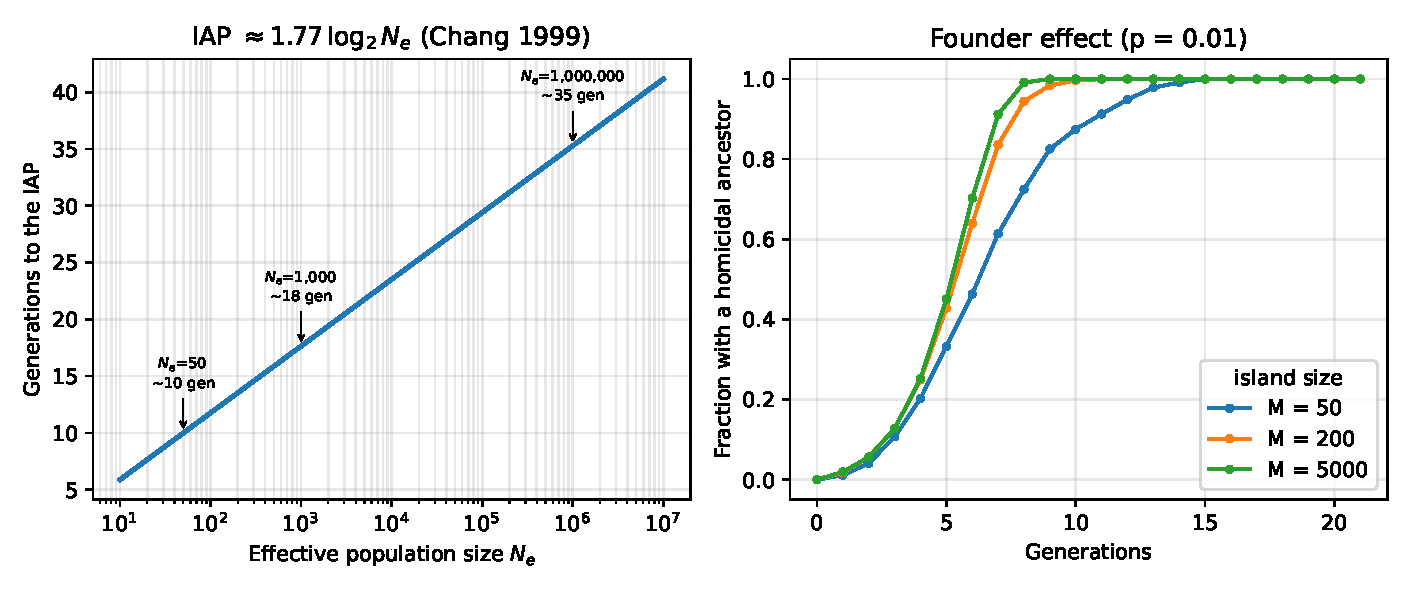
\includegraphics[width=0.92\textwidth]{fig_isolation_en.pdf}
\caption{Isolated populations. Left: generation of the IAP versus the effective
size $N_e$ ($\approx 1{.}77\log_2 N_e$). Right: fraction with a homicidal ancestor
per generation in closed populations of different size $M$ (founder effect,
$p=0{.}01$, Monte Carlo).}
\label{fig:isolation}
\end{figure}

\paragraph{Positioning and novelty.} This work does not claim a new mathematical
result: it is an expository \emph{synthesis} that combines already-known results
---the recent common ancestry of \citet{chang1999} and \citet{rohde2004}, and the
prevalence of lethal violence of \citet{gomez2016}--- to answer a concrete
existential question quantitatively. Its contribution is pedagogical and
integrative: it makes explicit, with reproducible code and sensitivity analysis,
a corollary that usually remains implicit in the genetic-genealogy literature.

\section{Conclusion}

The probability of having no homicidal ancestor is, under any realistic
parametrisation, indistinguishable from zero. The exponential growth of ancestors
and pedigree collapse suffice to make it minuscule within a few generations; the
identical ancestors point turns it into a practical certainty of an almost
deductive character. Therefore, \emph{it is essentially impossible for a living
human not to descend from at least one killer}. The existential intuition that
motivated this note is thus rigorously refuted.

\section*{On the nature of the data}
\addcontentsline{toc}{section}{On the nature of the data}
This work \emph{does not collect primary data}. It is worth distinguishing three
kinds of figures. (i) The \emph{empirical values} (prevalence of lethal violence,
IAP horizon, population size, generation length, etc.) are \emph{secondary}: they
come from external, peer-reviewed sources, cited in the text and traced one by
one ---with DOI and verbatim quotation--- in the file \texttt{EVIDENCE.md} of the
repository. (ii) The \emph{numerical results} (tables, figures and simulations)
do not depend on the author's authority but are \emph{reproducible}: they are
obtained by running the open code with fixed seeds. (iii) The \emph{model and its
derivations} are verifiable by mathematical inspection. In addition, the
parameters are taken as orders of magnitude and the conclusion is robust over wide
ranges (Sections~\ref{sec:param} and~\ref{sec:disc}), so it does not depend on any
single value. Consequently, verification of any claim is referred to its cited
source or to re-running the code, not to the author's testimony.

\section*{Reproducibility}
\addcontentsline{toc}{section}{Reproducibility}
All numerical results, tables and figures are generated by the code in the
\texttt{code/} directory (Python; see \texttt{requirements.txt}). The Monte Carlo
simulation uses fixed seeds, so its results are deterministic and reproducible.
This document is compiled with Tectonic (\texttt{tectonic main-en.tex}).

\section*{Data and code availability}
\addcontentsline{toc}{section}{Data and code availability}
The code, derived data and sources of this article are available in the project
repository (\url{https://github.com/JuanoLemos/paper-antepasado-asesino}) and are
permanently archived in Zenodo with DOI
\href{https://doi.org/10.5281/zenodo.20806914}{10.5281/zenodo.20806914}. The
traceability of each claim to its primary source is documented in the file
\texttt{EVIDENCE.md}. The code is distributed under the MIT licence and the text
and figures under CC-BY-4.0.

\section*{Competing interests}
\addcontentsline{toc}{section}{Competing interests}
The author declares no competing interests.

\bibliographystyle{plainnat}
\bibliography{refs}

\end{document}
